\documentclass[conference]{IEEEtran}
\IEEEoverridecommandlockouts
% The preceding line is only needed to identify funding in the first footnote. If that is unneeded, please comment it out.
\usepackage{cite}
\usepackage{amsmath,amssymb,amsfonts}
\usepackage{algorithmic}
\usepackage{graphicx}
\usepackage{textcomp}
\usepackage{xcolor}
\graphicspath{ {Resources/} }
\def\BibTeX{{\rm B\kern-.05em{\sc i\kern-.025em b}\kern-.08em
    T\kern-.1667em\lower.7ex\hbox{E}\kern-.125emX}}
\begin{document}

%\title{Simple Snake as testbed for reinforcement learning algorithms}
\title{Comparison of reinforcement learning algorithms on a Simple Snake testbed}

\author{\IEEEauthorblockN{Giovanni Gheriglio}
\IEEEauthorblockA{\textit{Alma Mater Studiorum} \\
\textit{University of Bologna}\\
Bologna, Italy \\
giovanni.gheriglio@studio.unibo.it}}

\maketitle

\begin{abstract}
Snake used to be a very popular mobile game in older Nokia phones. Its semplicity made it very easy to approach. This dissertation shows 
a simple implementation of the game to be used as testbed. Two different AI-agents from value approximation functions and policy gradient methods
are presented to test the environment.
\end{abstract}

\begin{IEEEkeywords}
snake, game, ddqn, a2c
\end{IEEEkeywords}

\section{Introduction}
Single-player Snake video games became popular with the rise of Nokia phones in the late 90s. 
The game was preloaded on the majority of their phones. As many 2D games, Snake has been used to test different reinforcement
learning approaches. Some versions of it used to be featured on the popular OpenAI Gym environment. 
This dissertation presents a simple version of the game and its structure. Two different agents are compared to test the environment.
One agent uses a \textit{value function approximation} algorithm with two networks and a replay buffer. The other agent adopts a \textit{actor-critic method} with 
the help of an advantage function to stabilize the training. The algorithms are briefly presented with their training specifications. In the end 
we'll show the results during training and subsequent tests.

\section{Background}
Snake is a single-player video game. The game is played on a two-dimensional square board. A snake is randomly placed on the board and is represented 
by a head and a body. The snake always moves horizontally or vertically. Its goal is to eat a fruit also placed randomly on the board. After the fruit gets
eaten the snake gets longer and another fruit spawns. At the same time the game score goes up. The game ends when the snake goes out of the board or when it hits
its own body.

\subsection{Environment implementation}
Our implementation is highly based on the original game. The board of choice is a 5x5 matrix. The snake and the fruits are placed randomly at each episode. There are
four possible actions the agent can take at each step: UP, RIGHT, DOWN, LEFT. Differently from the original game the snake is only made by its head. So it cannot get
longer after eating the fruit voiding the possibility of hitting against itself. \\
The environment offers the same basic methods OpenAI Gym's environments have: \textit{reset()}, \textit{step()}, \textit{render()}. The \textit{reset()} function
initializes the game board. Each element is assigned with one of three possible values:
\begin{itemize}
    \item 0 - \textit{empty}
    \item 1 - \textit{snake}
    \item 2 - \textit{fruit}
\end{itemize}
The \textit{step()} function takes the agent action evaluating the movement. In case the snake was going out of the board a variable \textit{done} is sent to the agent.
Both functions return the state of the game, which is made of three values:
\begin{itemize}
    \item Position of the snake on the board
    \item Position of the current fruit to eat
    \item Minimum number of actions for the snake to reach the fruit (relative distance)
\end{itemize}
The positions of the elements on the board are calculated according to this formula:
\[ element\_row * board\_rows + element\_column \]

The reward structure is set to mimic the game dynamics.
\begin{center}
\begin{tabular}{| c | c |}
    \hline
    \textbf{State} & \textbf{Reward} \\
    \hline\hline
    Lose & -1 \\
    \hline
    Standard movement for 30 consecutive steps* & - 0.1 \\
    \hline
    Standard movement & 0 \\
    \hline
    Eat fruit & +1 \\
    \hline
\end{tabular}
\end{center}

*\textit{This specific reward was necessary for avoiding the agent taking circular steps without any punishment.} \\
Despite the trivial nature of the game the number of possible states for a 5x5 matrix is about $3^{25}$.

\section{Experimental Algorithms}
In order to test our Snake environment we experimented with two radical approaches. In particular tests have been carried out with double DQN
as a value function approximation and A2C as an actor-critic method. To keep consistency for a true analysis both were trained with the same parameters:
\begin{itemize}
    \item \textit{discount factor} = 0.95
    \item \textit{learning rate} = 0.001
\end{itemize}
The optimizers and value loss functions used are also the same from \textit{tensorflow.Keras}:
\begin{itemize}
    \item \textit{optimizers.Adam}
    \item \textit{losses.mean\_squared\_error}
\end{itemize}

\subsection{DDQN}
Double DQN\cite{b1} is an improvement over the regular DQN algorithm with buffer replay. Instead of using only one network for action selection and action evaluation
there are two networks, one for each job. The network for action selection is called the \textit{Online network}. The one for evaluating is the \textit{Target network}.
The presence of the second network prevents the algorithm to overstimate action values. The two networks are identical.
In our case they are made of two hidden layers fully connected with 32 units each.

\subsection{A2C}
A2C is an \textit{Actor-Critic} method \cite{b2} with the use of an advantage function. It is made of two networks: a \textit{Policy network} and a \textit{State-value network}.
The actor uses the policy network to select the actions. At the same time the critic calculates the advantage function, which
measures how much better an action is compared to the average action in a given state.
The advantage applied to the backpropagation of the actor helps to stabilize learning.
In our tests the networks have a similar structure using two hidden layers fully connected with 32 units each. The weights are learned and updated separately.

\section{Experimental Results}
All tests are carried out using the Tensorflow library. In each algorithm the state gets preprocessed before being given to the networks. The preprocess
consists of a normalization of the values to [0, 1] and a conversion to tensor, through the function \textit{tf.convert\_to\_tensor}().
In order to be more memory efficient in the DDQN memory state values are saved as int.\\
Each episode has a maximum number of steps set to 300. If the agents make 30 consecutive steps without getting any fruit the episode ends
with a negative reward of -0.1.

\subsection{Training}
The two agents were trained for several episodes. DDQN was trained for 4000 episodes. While A2C was trained for 100000 episodes.
The \textit{Running average} shown in the following graphs is the average over the last 100 and 5000 scores respectively. The average is only meant as a guidance
for the progression in training.\\
As we can see from Fig.1 DDQN needs far less episodes to understand the game and achieve high scores. Regarding the A2C agent shown in Fig.2
the training is much slower. In addition the agent suffers from high variance in the scores achieved. Even when the agent starts
gaining confidence in the game it can get very poor scores, hence resulting in low average scores.\\
From a very early stage of training both agents seem to understand well the boundaries of the board. This is more noticeable in the
Fig.1 where the number of reached steps stops at 30 for several episodes. Efficiently eating the fruits is a skill both develop afterwards.

\begin{figure}[ht]
    \centering
    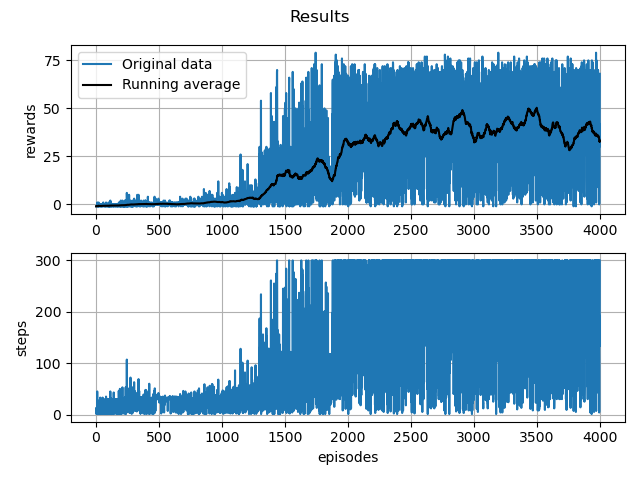
\includegraphics[scale=0.5]{training_snake_4000}
    \caption{DDQN Training}
\end{figure}

\begin{figure}[ht]
    \centering
    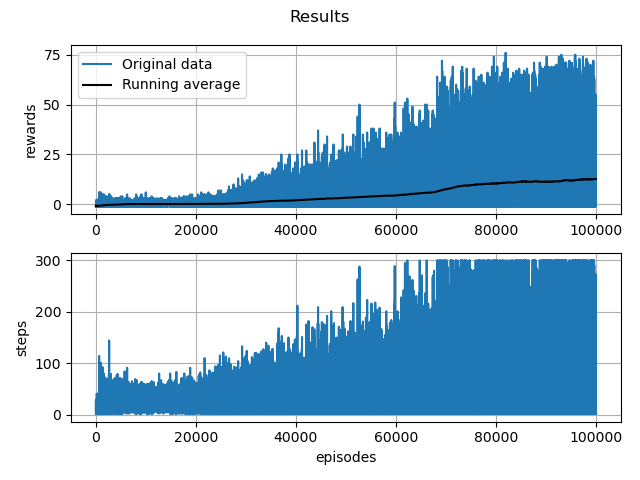
\includegraphics[scale=0.5]{training_snake_100000}
    \caption{A2C Training}
\end{figure}

\subsection{Agent performances}
Performances of the trained agents were tested on 100 consecutives runs of the game. This was made to flatten the differences created by the stochastic
placements on the board. The table below shows the results.

\begin{center}
    \begin{tabular}{| c | c | c | c |}
        \hline
        \textbf{Agent} & \textbf{Mean Score} & \textbf{Max Score} & \textbf{Training}\\
        \hline\hline
        DDQN & 24.99 & 75 & 4k episodes\\
        \hline
        A2C & 14.93 & 71 & 100k episodes\\
        \hline
    \end{tabular}
\end{center}

Both agents demonstrate to be very good at the game. The max scores show how the agents have become efficient in taking almost the minimum
number of steps to eat a fruit. Max scores are very similar. Although considering the mean values the trained A2C shows its limitation. This result
may be due to insufficient training or simply due to the more difficulties the agent finds in the environment tested.

\section{Conclusion}
Snake is a trivial videogame that is not as popular as it used to be. Although it still represents an ideal challenge for AI-agents. In our work we showed how a simple version
of it still makes a suitable testbed for comparing algorithms and networks. In particular the DDQN network proved significantly capable of mastering it. On the other
hand A2C agent achieved very good results with less robustness overall.

\nocite{*}
\begin{thebibliography}{00}
\bibitem{b1} Hado van Hasselt, Arthur Guez and David Silver, ``Deep Reinforcement Learning with Double Q-learning,'' 2015.
\bibitem{b2} Barto and Sutton ``Introduction to Reinforcement Learning,'' Chapter 13, Second Edition, MIT Press 2018.
\end{thebibliography}

\end{document}